\chapter{Degrees}
Rishnak asked Ajur whether he knew about graphs and trees in mathematics. Ajur jumped up and down and proclaimed that he knew all about graph theory. He continued that graphs are often used to  represent relations of a set of objects. He enthusiastically stated that the famous mathematician Euler was the father of graph theory. He was eager to show off his knowledge and described the famous  K\"{o}nigsberg bridge problem.  K\"{o}nigsberg (in modern day Russia) was on the banks of the Pregel river.  There were seven bridges across this river, connecting the two sides of the river and two islands. Ajur drew a graph of this on a piece of paper he was carrying.
\begin{figure}
\begin{center}
\includegraphics[width=0.6\textwidth]{konigsberg.JPG}
\caption{A Graph representing K\"{o}nigsberg Bridge. Vertices 1 and 3 are islands and 0 and 2 are the two riverbanks.}\label{kon}
\end{center}
\end{figure}

He continued that the problem was to start from the vertex labeled 0 and go through all bridges once and only once and return to the starting vertex 0. Ajur could not contain his enthusiasm and asked Rishnak how to do it. Rishnak gently reminded Ajur that he was the one asking questions and Ajur just had to respond with correct responses. Ajur nodded his head enthusiastically.

 Since this was the first time, Rishnak told Ajur that he was going to ask Ajur a series of questions and observe whether his curses could be lifted.
 
 Rishnak then asked Ajur, ``in a class of 33 students, what is the maximum and minimum number of friends a student can have?"\footnote{Being friend is a mutual relation, i.e. if A is a friend of B, then B is a friend of A. A student cannot be a friend to herself!}
 
 Ajur nonchalantly replied that the maximum number is 32 and the minimum number is 0.
 
 Rishnak then asked Ajur ``will there be a student in a class having 32 friends and a student having 0 friends?"
 
 Ajur smiled to himself that Rishnak seems like a clever ghost; Ajur replied, ``how is that possible --- if a student has 32 friends, so she is friends with everyone else, then everyone else has at least one friend. 
 So there cannot be a 
 student with 0 friends. Similarly if there is a student with 0 friends, there are only 32 students remaining and another student can have at most 31 friends."
 
 Rishnak was pleased to have found someone who seemed to have the ability to help him and the questioning continued. ``Can all the 33 students have a distinct number of friends?"
 
 Ajur responded immediately saying it is not possible because there are 33 distinct students, and the distinct number of friends the class can have is $\{0,1,2,\cdots,32\}$. There are 33 numbers in this, but alas it contains both students with 32 friends and with 0 friends. Ajur just had told Rishnak that it is not possible to have a student with 32 friends and another student with 0 friends.
 
 Rishnak asked Ajur, ``can there be just two students having the same number of friends, with the others all having distinct numbers of friends?" Rishnak further added that all of the students have at least one friend.
 
Ajur wanted to reason it out. He knew that the maximum number can only be 32, and the minimum has to be 1, so there are 32 distinct numbers. But there are 33 students. So by the pigeon hole principle --- if there are more pigeons than boxes, then one box contains at least two pigeons --- there have to be two students with the same number of friends.  He then reasoned about what the numbers could be. He matched 32 with 1: that is, the student having one friend has to be a friend of a student with 32 friends. Then he matched 2 with 31: the student with 2 friends has to be a friend of a student with 32 friends and a student with 31 friends. Continuing this argument, he matched 3 with 30, 4 with 29, $\cdots$, 15 with 18 and 16 with 17. We have an even number of students accounted for but an odd number of total students. That means there are two students having the same number of friends.

Rishnak posed the next question: He asked 5 students in a class of 6 students how many friends each of them have and they all gave distinct numbers greater than 0. How many friends does the student who was not asked have?

Ajur thought about this. If all the five students had given distinct numbers and they were greater than 0, they had to be $\{1,2,3,4,5\}$. Let the students be A(pu), B(art), C(arla), D(uma), E(rnie) having 5, 4, 3, 2 and 1 friends respectively. Let F(ermat) be the sixth student. A is friends with B, C, D, E and F. B is friends with C, D and F. B is already friends with A and E has only one friend, namely A. Now C is friends with F. C is already friends with A and B, and D and E have their friends quota counted already. 
Now it is easy to see that F(ermat) has exactly 3 friends, namely A, B and C.

Ajur drew the following graph as in Figure \ref{dg2}.

\begin{figure}
\begin{center}
\includegraphics[width=0.6\textwidth]{graphstory1-1.JPG}
\caption{A Graph with 6 students and 5 students having 5, 4, 3, 2 and 1 friends}\label{dg2}
\end{center}
\end{figure}

Rishnak was impressed, but wanted to test Ajur further. He asked whether there can an be odd number of students having odd number of friends. Ajur said that it is impossible as the sum of all numbers of friends across all students has to be even. He reasoned that if A is a friend of B, then this friendship is counted twice. Hence the sum of all friends of students is even. We know that the students having an even number of friends will contribute an even number of friendships. This in turn implies that the number of students having an odd number of friends has to be even.


Rishnak started asking, ``can you draw a graph of a class with 5 students respectively having 1, 2, 2, 2 and 1 friends?"

Ajur whipped up the graph drawn in Figure \ref{dg3}. 

\begin{figure}
\begin{center}
\includegraphics[width=0.6\textwidth]{graphstory1-2.JPG}
\caption{A Graph with 5 students having 2, 2, 2, 1 and 1 friends}\label{dg3}
\end{center}
\end{figure}

Rishnak asked whether one can draw another graph having the given friends list.\footnote{Hakimi has given a method of constructing a graph with a given degree sequence}

Ajur took no time to respond and drew another graph as in Figure \ref{dg4}.

\begin{figure}
\begin{center}
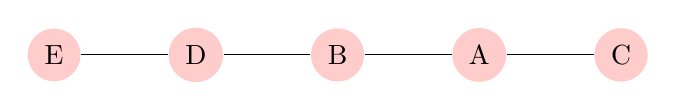
\begin{tikzpicture}
  [scale=.6,auto=left,every node/.style={circle,fill=red!20}]
  \node (n1) at (0,0) {E};
  \node (n2) at (3,0)  {D};
  \node (n3) at (6,0)  {B};
   \node (n4) at (9,0)  {A};
  \node (n5) at (12,0)  {C};
  \foreach \from/\to in { n1/n2,n2/n3,n3/n4,n4/n5}
    \draw (\from) -- (\to);

\end{tikzpicture} %\includegraphics[width=0.6\textwidth]{graphstory1-3.JPG}
\caption{Another Graph with 5 students having 2, 2, 2, 1 and 1 friends}\label{dg4}
\end{center}
\end{figure}

Jura was waking up and wanted to play with Ajur. Rishnak was happy to see the answers that Ajur gave. He saw a ray of hope that his curse could be lifted. 

\textbf{Question for the first day:}  Provide a degree sequence that is the degree sequence of only one graph? (You can ignore the labels on vertices.)

\textbf{Answer:} Ajur said that the degree sequence of all 0's have only one graphical realization!

\textbf{Followup Question:}Rishnak said he agreed to Ajur's answer. Is there a degree sequence with only one graph realizing it and having one or mode edges?

\textbf{Answer:} Ajur responded for a sequence of even length, a degree sequence, of $1,1,\cdots, 1$ will be realized by a unique graph.

He showed an example with $1,1,1,1,1,1,1,1$ in the following Figure \ref{daya1}

\begin{figure}
\begin{center}
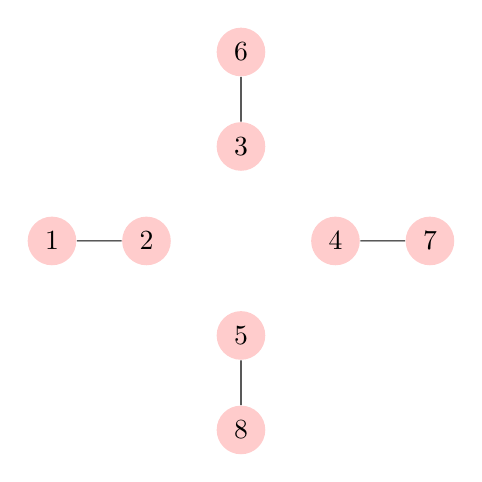
\begin{tikzpicture}
  [scale=.6,auto=left,every node/.style={circle,fill=red!20}]
  \node (n1) at (1,7) {1};
  \node (n2) at (3,7)  {2};
  \node (n4) at (7,7) {4};
  \node (n7) at (9,7)  {7};
  \node (n6) at (5,11)  {6};
   \node (n3) at (5,9) {3};
   \node (n5) at (5,5) {5};
   \node (n8)  at (5,3) {8};
  \foreach \from/\to in {n1/n2,n3/n6,n4/n7,n5/n8}
   \draw (\from) -- (\to);

\end{tikzpicture}
\caption{ Unique Graph with degree sequence 1,1,1,1,1,1,1,1 }\label{daya1}
\end{center}
\end{figure}

Rishnak told Ajur to come back the next night, and he disappeared in a cold mist.